\documentclass[11pt]{article}
\usepackage[margin=1in]{geometry}
\usepackage{amsmath,amssymb,amsthm}
\usepackage{graphicx}
\usepackage[hidelinks]{hyperref}
\usepackage{microtype}

\title{\bfseries Orbital Dragons to Hunt Cryptids:\\
Utilizing Non-Euclidean Geometry to Solve Busy Beaver}
\author{Enan Srivastava}
\date{DeepMath 2026 --- Extended Abstract}

\newtheorem{theorem}{Theorem}
\newcommand{\Halts}{\mathsf{RawHalts}}
\newcommand{\Safe}{\mathsf{SafeMetaOrbit}}

\begin{document}
\maketitle

\begin{abstract}
The busy beaver value $BB(n)$ is the longest finite runtime of any
$n$-state Turing machine started on a blank tape. $BB(5)$ was settled
in 2024 with a computer-checked proof. $BB(6)$ is blocked by a handful
of machines whose tapes secretly run Collatz-style arithmetic; nobody
can prove whether they stop. We study two of these machines. Our
approach is empirical first: we log the machine's behavior as a
sequence of events, embed the event data in logarithmic, simplex, and
hyperbolic coordinates, and find that the dynamics are piecewise
affine in a five-integer state. We then prove this description correct
in the Lean proof assistant, down to the machine's individual steps and
with a minimal axiom footprint. The result is a machine-checked
theorem: if a simple five-integer recurrence never enters an explicit
finite set of bad configurations, the machine never halts. We also
prove the converse pressure: entering a bad configuration forces the
machine to halt. The open problem is thereby moved, without loss, from
a Turing machine to a short arithmetic recurrence. We then derive the
recurrence's renewal map in closed form, show its fatal set is a
width-five window around the diagonal, and close the two mechanical
proof routes with computational evidence: no congruence invariant up to
modulus 384 excludes the window, and the branch dynamics has
exponential factor complexity, so it is not conjugate to a rotation.
Every empirical claim is validated against $10^{9}$ raw machine steps,
and the recurrence is tested for $10^{8}$ iterations.
\end{abstract}

\section{The problem, from zero}
A Turing machine here is a finite table: six control states, a tape of
0s and 1s, and for each (state, read symbol) pair an instruction ---
write a bit, move left or right, change state --- or nothing. If the
table has no instruction for the current situation, the machine halts.
$BB(n)$ asks: among all $n$-state tables that eventually halt from the
all-zero tape, what is the longest runtime? The function is
noncomputable, so each new value is won machine by machine: every table
either halts (run it) or must be \emph{proven} to run forever.

The bbchallenge collaboration settled $BB(5)=47{,}176{,}870$ with a
proof checked in the Rocq proof assistant \cite{coqbb5,deciders}. At
six states a residual set of machines defeats all known automated
deciders. The community calls them cryptids. The reason they are hard
is concrete: their tape dynamics implement iterated arithmetic maps of
the same character as the Collatz ($3x{+}1$) map --- deterministic
integer maps where parity decides the next move, and where the question
is whether one specific orbit ever hits a small bad set. The strongest
known result for such maps is Tao's: \emph{almost all} Collatz orbits
reach almost bounded values \cite{tao-collatz}. That theorem is about
typical orbits. Busy beaver questions need the worst case: one orbit,
followed forever. No general tool exists for that, which is why each
cryptid is studied on its own terms.

We work on two six-state cryptids, a mirror-image pair we call
dossier-2 and dossier-3. Machine one is
\texttt{1RB1RC\_1LC1LC\_1RE0LD\_1LB1RF\_---1RA\_0RD1RD} in the standard
table notation.

\section{What we do}
Our method has three stages. Watch, compress, certify.

\textbf{Watch.} We run the machine and record only the moments that
matter. For these machines there is a natural clock: a recurring
configuration we call a spawn entry. Between two spawn entries the
machine performs one bounded ``episode'' of work. Sampling at spawn
entries turns a raw trajectory of $10^{9}$ steps into a clean sequence
of a few million events.

\textbf{Compress.} At every spawn entry the tape has the same form: a
solid block of 1s with exactly two 0-cells (``holes'') inside it. So
the whole configuration is five integers: the block's two endpoints
$l, r$, the hole positions $h_1, h_2$, and a tag. We write
$a = h_1 - l$, $b = h_2 - h_1$, $c = r - h_2$ for the three gap
lengths. Plotted in raw coordinates, the event data looks like growth
curves with no visible law (Figure~\ref{fig:std}). Plotted in the
right coordinates the same data is piecewise linear: componentwise
$\log(1{+}x)$ straightens each regime, the projective simplex
$(a,b,c)/(a{+}b{+}c)$ removes scale, and hyperbolic and spherical
renderings of those two charts expose the orbit's nested renewal
structure (Figure~\ref{fig:charts}). Straight segments
are one regime; corners are regime changes. These coordinate choices
are standard elsewhere: the log map is the tropical limit of algebraic
geometry --- historically, a dequantization, the $\hbar \to 0$ limit
of a quantum calculus \cite{viro,litvinov}; the simplex normalization
with its Fisher--Rao metric is the classical face of quantum state
geometry, made literal by the amplitude map $p \mapsto \sqrt{p}$; and
shape-versus-scale is the hyperbolic geometry used for hierarchical
data \cite{nickel-kiela}. The underlying view of
a Turing machine as a dynamical system goes back to Moore and
K\r{u}rka \cite{moore,kurka}.

\begin{figure}[t]
\centering
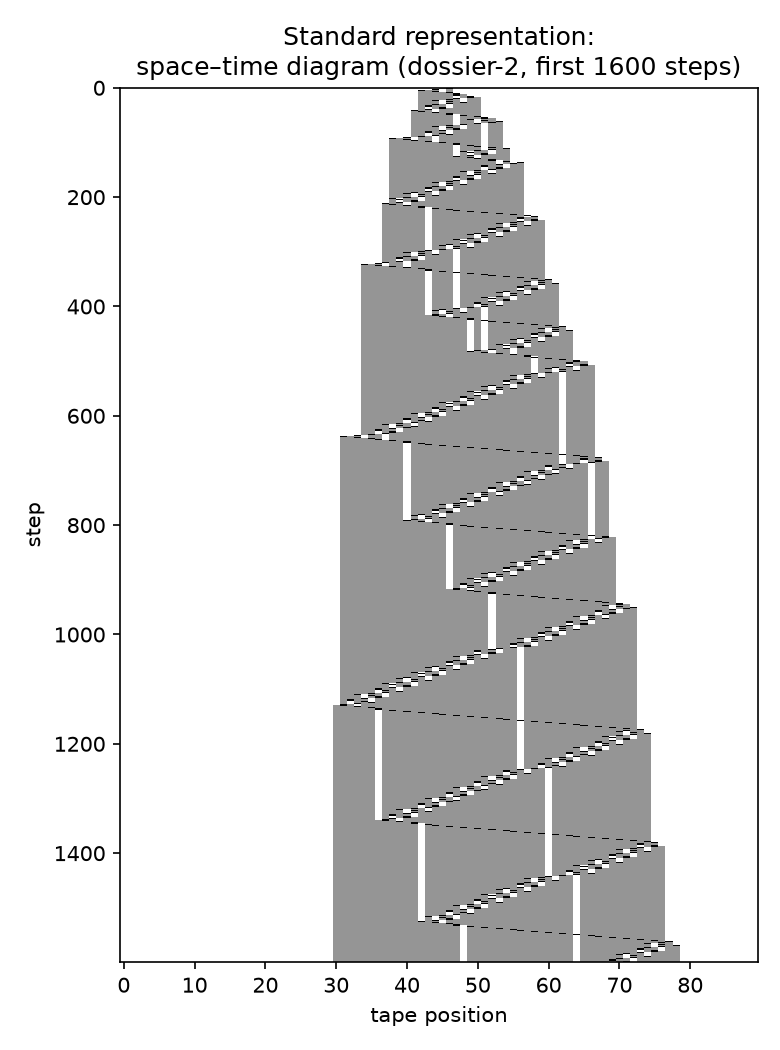
\includegraphics[height=2.4in]{fig1_spacetime.png}
\caption{Raw view: the machine's first 1{,}600 steps (dark = 1s, one
row per step). Nothing about the long-run law is visible here.}
\label{fig:std}
\end{figure}

\begin{figure}[t]
\centering
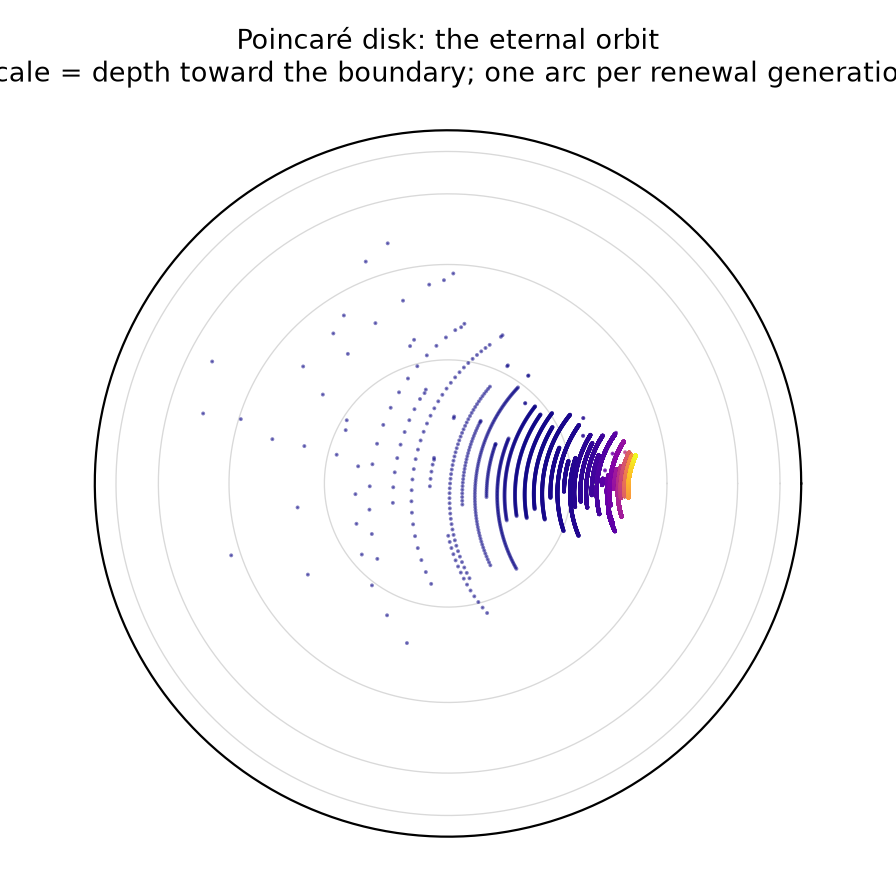
\includegraphics[height=2.55in]{fig5_poincare.png}\hfill
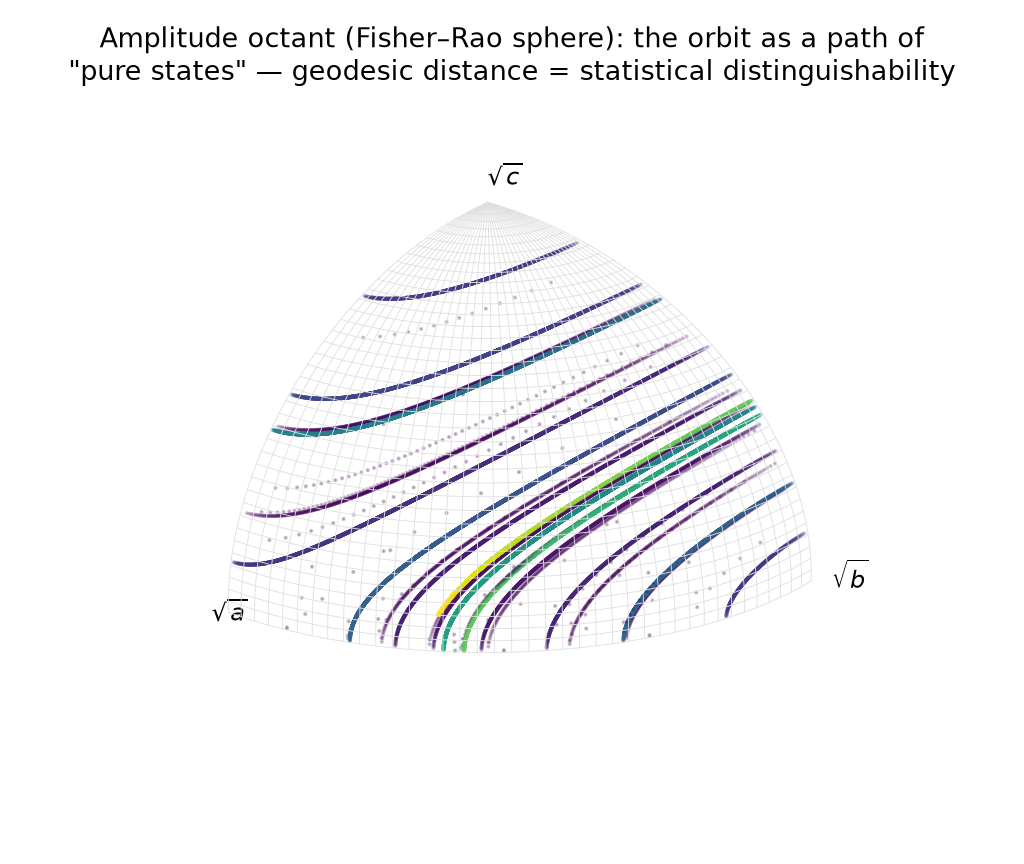
\includegraphics[height=2.55in]{fig6_fisher_rao.png}
\caption{The same machine, 100{,}050 events, in two non-Euclidean
coordinate systems. Left: the Poincar\'e disk --- shape runs along the
boundary direction, log-scale is hyperbolic depth, and each renewal
generation of the orbit sits one nested arc deeper. Right: the
amplitude octant --- the normalized state $(a,b,c)/(a{+}b{+}c)$ mapped
by $p \mapsto \sqrt{p}$ onto the Fisher--Rao sphere, so the orbit
becomes a path whose geodesic length measures statistical
distinguishability. Straight arcs are single regimes; corners are
regime changes.}
\label{fig:charts}
\end{figure}

\textbf{Certify.} The picture suggests a law; the law must then be
proven about the actual machine, or it is only a picture. We first
validate it empirically and fail-closed: a predictor that knows the
conjectured law must reproduce every event --- exact positions, exact
tape --- over $10^{9}$ raw steps per machine, and any miss aborts. It
reproduces all of them. We then prove the law in Lean~4, using only the
kernel's minimal axioms (\textsf{propext}, \textsf{Quot.sound}; no
classical choice). The certified account consists of: seven theorems,
one per episode type, each giving the episode's exact step count,
exact output shape, and safety; two inductions that handle the
episodes' unbounded middle parts; a concrete certificate for the
machine's startup (235 steps for one machine, 2{,}044 for the other);
and a transport theorem showing that a five-integer function
$\mathsf{metaStep}$, iterated from the startup state, predicts the
machine forever.

\section{The result}
Halting, for these machines, can only happen one way: a specific
control state must read a 0 with another 0 beside it. The certified
episode theorems show this situation never arises while the
five-integer iteration stays inside an explicit guarded region. Writing
$\Safe$ for the statement that the iteration never leaves that region:

\begin{theorem}
For each machine, checked by the Lean kernel at axioms
$\{\mathrm{propext},\mathrm{Quot.sound}\}$:
$\ \Safe \rightarrow \lnot\Halts(\mathsf{blankStart})$.
\end{theorem}

Two facts make this reduction meaningful rather than cosmetic. First,
it is complete: startup, one exceptional episode, and every future
step of the machine are covered by theorems, so nothing about the
machine remains to be understood --- only the arithmetic. Second, it is
sharp: we constructed the configurations just outside the guarded
region and ran the machine from them; it halts within about fifty
steps. Leaving the region is not merely unproven-safe. It is fatal.
So $\Safe$ \emph{is} the halting problem, restated as arithmetic.

What kind of arithmetic? Inside the main regime the iteration is
$(a,b,c) \mapsto (a{+}6,\,b{-}2,\,c{-}2)$, so $\gamma = c - b$ is
conserved while the counters drain. When $b$ or $c$ runs out, a
renewal move re-seeds the triple by subtracting and swapping counters,
with parity choosing the branch --- part Euclidean algorithm, part
Collatz. Figure~\ref{fig:gamma} shows the renewal process as its own
dynamical system: the return map of $\gamma$, with the fatal values
$\gamma \in \{1,3,5\}$ marked. The recurrence avoids the band for $10^{8}$
iterations (about $10^{15}$ machine steps). Proving it does so forever
is the open problem, now in a form a number theorist can hold in one
hand.

We characterized that problem further. Sampling the orbit at its
renewal section reduces the whole dynamics to a two-counter map,
verified exactly against the certified orbit: with
$(\alpha,\beta) = (6, a{-}1)$ or $(9, a{-}2)$ by the parity of $a$,
$$R(a,b) = \begin{cases}
(a+6,\ b-3) & b \text{ even},\\
(\alpha + 3(b-3),\ \beta - (b-3)) & b \text{ odd},\ b < \beta,\\
(\alpha + 3\beta + 3,\ b - \beta - 4) & b \text{ odd},\ b > \beta.
\end{cases}$$
Its fatal set is geometrically simple: death occurs exactly when the
two counters arrive almost equal ($b - \beta \in \{1,3,5\}$, plus
two boundary cases). Two mechanical proof routes are then closed by
computation. A sound residue-abstraction search finds a genuine mod-3
conservation law but shows that no congruence invariant up to modulus
$384$ excludes the fatal window. And the branch-symbol sequence has
factor complexity growing like $1.6^{n}$ --- a rotation coding would
give $n+1$ --- so the dynamics is not conjugate to a rigid system, and
continued-fraction rigidity arguments do not apply as stated. Over
$10^{5}$ renewals the orbit's minimum distance above the fatal window
is $4$: it grazes death and survives, so no proof can rely on a
structural buffer. What remains is a pointwise avoidance statement for
a pseudorandom multiplicative map --- the Collatz situation --- with
three mitigations: the map is explicit and total, the fatal set is a
finite union of lines near the diagonal, and the certified reduction
stands under any future argument. The natural next language is
hyperbolic: renewal steps are integer $2{\times}2$ matrix moves, and a
near-tie of the counters is a cusp excursion on the modular surface, so
the conjecture asks that a specific geodesic avoid three explicit
horoballs forever \cite{series}.

\begin{figure}[t]
\centering
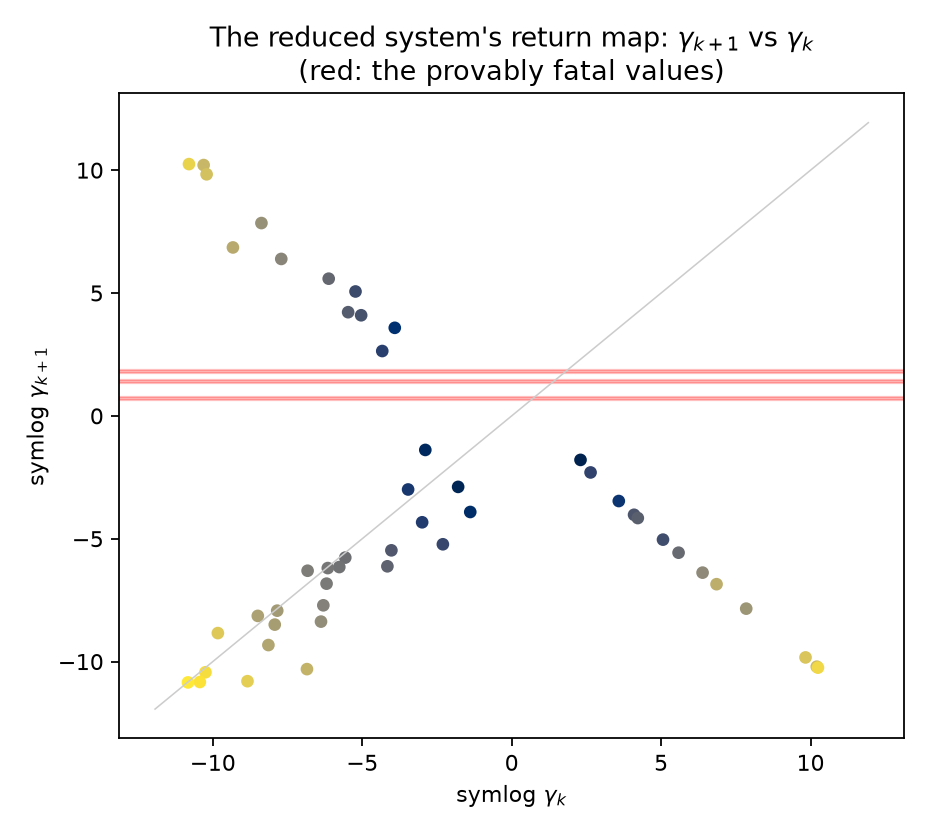
\includegraphics[width=0.62\textwidth]{fig8_returnmap.png}
\caption{The reduced problem, as a dynamical system in its own right:
the return map of the renewal invariant, $\gamma_{k+1}$ against
$\gamma_k$ (symlog axes), over the first fifty renewals. The red bands
are the values proven fatal. The conjecture: the map's orbit never
lands in a band.}
\label{fig:gamma}
\end{figure}

\section{Why this may interest this community}
Two reasons. The first is the workflow. This project is an instance of
the emerging human--AI--kernel pattern in mathematics --- AI systems
draft and compile proofs at scale, a proof kernel arbitrates, humans
own claims --- the pattern of Tao's Equational Theories Project and the
new Palomar registry for Lean-verified results \cite{etp,palomar}. All
of our Lean was drafted by an AI assistant from validated empirical
specifications; the kernel checked roughly fifteen thousand lines; the
generators are convenience, not trust surface. The second reason is
methodological kinship. Finding that a high-dimensional trajectory is
governed by a low-dimensional piecewise-affine law, by choosing
coordinates in which the structure is linear, is the daily business of
representation learning. Here the same move is carried one step
further: the discovered representation is not evaluated on held-out
data but proven exactly correct, step by step, against the system that
generated it.

\paragraph{Scope.} We claim no unconditional non-halting result. The
coordinate charts guide discovery and exposition; no theorem depends on
them. Empirical horizons are what we ran, not what is true.

\paragraph{Acknowledgments.} The Lean developments, empirical
validation, and proof generators were built in collaboration with an AI
assistant (Claude, Anthropic). Every proof is checked by the Lean~4
kernel at the stated axioms.

\begin{thebibliography}{9}\small
\bibitem{coqbb5} The bbchallenge Collaboration.
Determination of the fifth Busy Beaver value. arXiv:2509.12337.
\bibitem{deciders} The bbchallenge Collaboration.
Turing machine deciders, part I. arXiv:2504.20563.
\bibitem{tao-collatz} T.~Tao. Almost all orbits of the Collatz map
attain almost bounded values. arXiv:1909.03562.
\bibitem{moore} C.~Moore. Generalized shifts: unpredictability and
undecidability in dynamical systems. \emph{Nonlinearity} 4 (1991).
\bibitem{kurka} P.~K\r{u}rka. On topological dynamics of Turing
machines. \emph{Theoret.\ Comput.\ Sci.} 174 (1997).
\bibitem{viro} O.~Viro. On basic concepts of tropical geometry.
\emph{Proc.\ Steklov Inst.\ Math.} 273 (2011).
\bibitem{litvinov} G.~Litvinov. Maslov dequantization, idempotent and
tropical mathematics. \emph{J.\ Math.\ Sci.} 140 (2007).
\bibitem{nickel-kiela} M.~Nickel and D.~Kiela. Poincar\'e embeddings
for learning hierarchical representations. NeurIPS 2017.
\bibitem{series} C.~Series. The modular surface and continued
fractions. \emph{J.\ London Math.\ Soc.} 31 (1985).
\bibitem{etp} T.~Tao et al. The Equational Theories Project.
arXiv:2512.07087.
\bibitem{palomar} T.~Tao. Palomar: a registry of Lean-verified
mathematics, 2026. \texttt{palomar-registry.org}.
\end{thebibliography}

\end{document}
